\chapter{Introduction} \label{chap:introdcution}

 Chapter \ref{chap:introdcution} provides a brief summary on some basic \LaTeX{} elements to be used in a thesis. A comprehensive literature review on [your topic] is presented in Chapter \ref{chap:literature}. Bla bla bla ....
 
 \section{Figure and Table}  \label{sec:FigureAndTable}

 Text body of the Section \ref{sec:FigureAndTable}.
 
 \subsection{Figure}  \label{subSec:Figure}

 
 A figure example is shown in Figure \ref{fig:Compare}.
 
 %%%%%%%%%%%%%%%% begin figure %%%%%%%%%%%%%%%%%%%
 \begin{figure}
     \begin{center}
         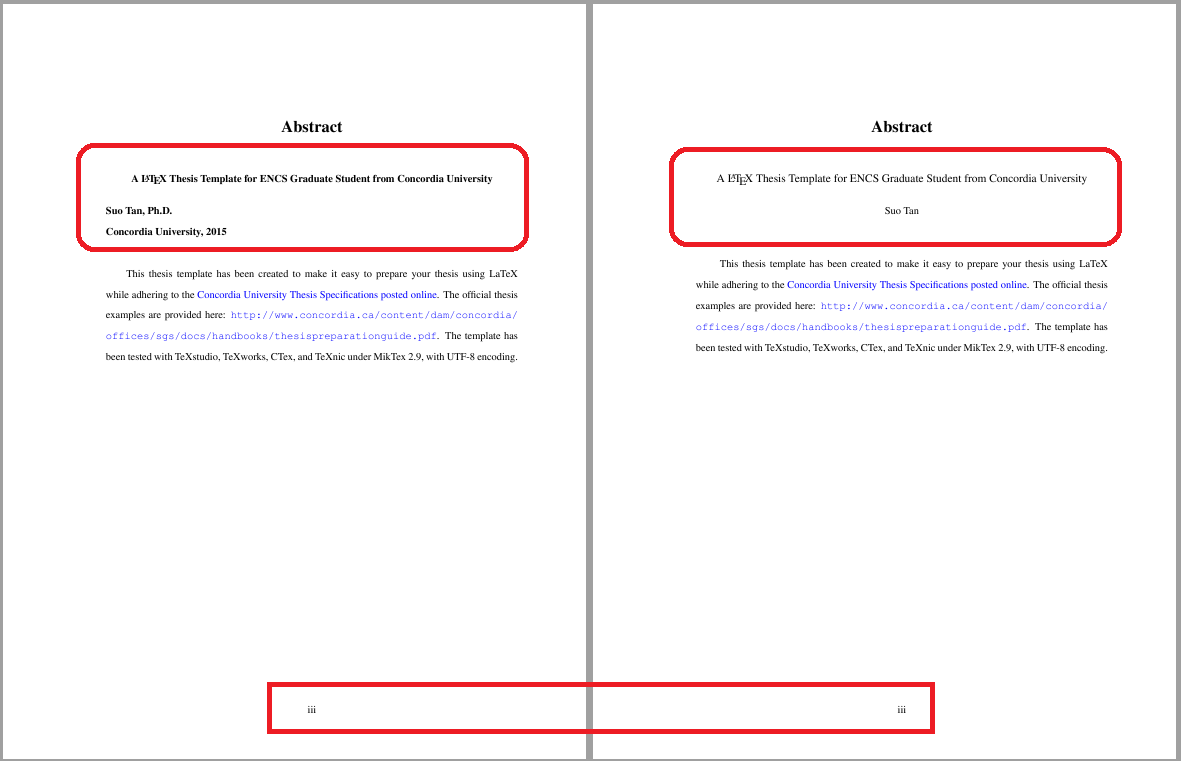
\includegraphics[scale=0.6]{Compare}  %it is suggested to using scale to zoom figures without distortion
        \end{center}
        \caption{An illustration of requirement compliance.}
        \label{fig:Compare}
    \end{figure}
%%%%%%%%%%%%%%%% end figure %%%%%%%%%%%%%%%%%%%
    
    
\subsection{Table}  \label{subSec:Table}
    
 Table \ref{table:ROM_elements} illustrates a very complex table with figures in its cells.
 
 \begin{table}[htp]
     \small{
         \caption{Elements defined for the ROM \citep{Zeng:2008}.}
         \begin{center}
             \label{table:ROM_elements}
             \begin{tabular}{p{1.3cm} p{1.8cm} p{2.1cm} p{4.5cm}} \hline \hline
                 \multicolumn {2}{c}{Type} &  Graphic Representation  & \multicolumn {1}{c}{Description} \\\hline
                 \multirow {3}*{Object} & Object & \hfil \raisebox{-0.35cm}{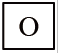
\includegraphics[scale=.5]{FigInTable1_1}} \hfil & Everything in the universe is an object \\
                 & Compound Object & \hfil \raisebox{-0.5cm}{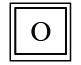
\includegraphics[scale=.5]{FigInTable1_2}} \hfil & It is an object that includes at least two objects in it\\\hline
                 \multirow {7}*{Relation} &  Constraint Relation & \hfil \raisebox{-0.6cm}{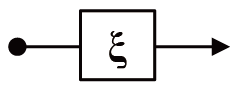
\includegraphics[scale=.4]{FigInTable1_3}} \hfil & It is a descriptive, limiting, or particularizing relation of one object to another\\
                 & Connection & \hfil \raisebox{-0.45cm}{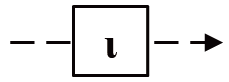
\includegraphics[scale=.4]{FigInTable1_4}} \hfil & It is to connect two objects that do not constrain each other \\
                 & Predicate Relation & \hfil \raisebox{-0.6cm}{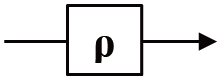
\includegraphics[scale=.4]{FigInTable1_5}} \hfil & It describes an act of an object on another or that describes the states of an object \\\hline \hline
                \end{tabular}
            \end{center}
        }
    \end{table}
    
    
\section{Itemized examples using list structures in \LaTeX{}}
\label{SubSec.:bullet}

Item list using ``\texttt{itemize}" structure are given below:

% itemize style 
\begin{itemize} 
    
    \item  Use bold/italic for emphasis, but keep its use to a minimum. Avoid using underlining in your paper.
    \item  Use a consistent spelling style throughout the paper (US or UK).
    \begin{itemize}  % level 2 items
        \item  Use double quotes.
        \item  Use \%, not percent.
        \item  Do not use ampersands (\&) except as part of the official name of an organization or company.
    \end{itemize}
    \item  Keep hyphenation to a minimum. Do not hyphenate `coordinate' or `non' words, such as `nonlinear'.
    
\end{itemize}

The following are using ``\texttt{enumerate}" structure:

% enumerated style 
\begin{enumerate} 
    
    \item  For complete or near complete sentences, begin with a capital letter and end with a full stop.
    \item  For short phrases, start with lower case letters and end with semicolons.
    
\end{enumerate}

    
\section{Algorithm}
    
    The pseudo code shown in Algorithm \ref{alg:myAlgo} describes the proposed algorithm.
    
    \begin{algorithm}
        \small{
            \caption{Calculate the probability of $G$}\label{alg:myAlgo}
            \begin{algorithmic} [1]
                \Require $p \in [0,1]$, $G$
                \Ensure None
                \For{$i = 0 \to 2^d-1$}\Comment{$d$ is an integer} 
                \If{$n(\nu_i) = 0$}
                \If{ $x < p$}  \Comment{$x$ is a normal distribution number in the range of $[0,1]$}
                \State Occupy $v_i$ site with probability $p$ 
                \EndIf
                \EndIf
                \EndFor
            \end{algorithmic}}
        \end{algorithm}
        
        
  \section{Equation}
        \label{section:equation}
        
        An equation example is shown in Eq. \ref{equ:enc}.
        
        \begin{equation}\label{equ:enc}
        f(ENC)=\int_0^{1}(e^{x}+x^{2})
        \end{equation}
        
\section{Quotations}
        \label{subSec:quotation}
        
        \begin{quote}
            ``It was easier in the beginning when there was only the RED-camera, but now, after RED, it just continuous. And all the different manufacturers, they cannot agree upon what is the standard file format, codec, or compression algorithms, and so on. It is a jungle."
        \end{quote}
        \begin{flushright} CEO, Full Name (Company A) \end{flushright}
        

\section{Citations}
        \label{subSec:Citations}
        
        It is suggested that you choose ``\textbf{$\backslash$citet}" and/or ``\textbf{$\backslash$citep}" to cite references. The ``\textbf{$\backslash$citet\{key\}}" gives you a format of  ``\textbf{Name (1990)}", whileas ``\textbf{$\backslash$citep\{key\}}" delivers a format of ``\textbf{(Name, 1990)}". For example, \citet{Wang&Zeng:2009} extended their research from \citep{Zeng:2008}.
        


        